%==============================================================================
% SJCET Literature Review Beamer Template (Final Corrected)
% Compile with pdfLaTeX (run twice for page numbers)
%==============================================================================
\documentclass[aspectratio=169,11pt]{beamer}

%------------------------------------------------------------------------------
% Packages
%------------------------------------------------------------------------------
\usepackage[utf8]{inputenc}
\usepackage[T1]{fontenc}
\usepackage{graphicx}
\usepackage{booktabs}
\usepackage{array}
\usepackage{xcolor}
\usepackage{tikz}
\usetikzlibrary{positioning,arrows.meta,calc,fit,backgrounds}
\usepackage{fontawesome5}
\usepackage[most]{tcolorbox}

%------------------------------------------------------------------------------
% Theme & Colors
%------------------------------------------------------------------------------
\usetheme{Boadilla}
\usefonttheme{professionalfonts}
\setbeamertemplate{navigation symbols}{}
\setbeamertemplate{frametitle continuation}{}

\definecolor{SJCETblue}{RGB}{25, 55, 95}
\definecolor{SJCETgold}{RGB}{184, 134, 11}
\definecolor{DarkGray}{RGB}{80, 80, 80}

\setbeamercolor{structure}{fg=SJCETblue}
\setbeamercolor{frametitle}{fg=SJCETblue,bg=white}
\setbeamercolor{title}{fg=SJCETblue}
\setbeamercolor{block title}{fg=white,bg=SJCETblue!90}
\setbeamercolor{block body}{bg=gray!8,fg=black}

\setbeamertemplate{itemize items}[circle]
\setbeamercolor{itemize item}{fg=SJCETblue}
\setbeamercolor{itemize subitem}{fg=SJCETblue}

% MAKE ALL FRAME TITLES BOLD
\setbeamerfont{frametitle}{series=\bfseries}

%------------------------------------------------------------------------------
% Footer: Solid SJCETblue bar, white text, full college name
%------------------------------------------------------------------------------
\setbeamercolor{author in head/foot}{bg=SJCETblue,fg=white}
\setbeamercolor{date in head/foot}{bg=SJCETblue,fg=white}

\setbeamertemplate{footline}{%
  \leavevmode%
  \hbox{%
    \begin{beamercolorbox}[wd=.80\paperwidth,ht=3.4ex,dp=1.3ex,leftskip=0.5cm,colsep=0pt]{author in head/foot}%
      \usebeamerfont{author in head/foot}%
      \small St. Joseph's College of Engineering and Technology, Palai%
    \end{beamercolorbox}%
    \begin{beamercolorbox}[wd=.20\paperwidth,ht=3.4ex,dp=1.3ex,rightskip=0.5cm,colsep=0pt]{date in head/foot}%
      \usebeamerfont{date in head/foot}%
      \raggedleft\small\textbf{\insertframenumber{} / \inserttotalframenumber}%
    \end{beamercolorbox}%
  }%
}

%------------------------------------------------------------------------------
% Document Info
%------------------------------------------------------------------------------
\title[]{}
\author{}
\institute{}
\date{}

%==============================================================================
\begin{document}
%==============================================================================

%------------------------------------------------------------------------------
% TITLE PAGE  (FIXED: date visible, tighter spacing, no center env padding)
%------------------------------------------------------------------------------
{
\setbeamertemplate{footline}{}
\setbeamertemplate{headline}{}
\begin{frame}[plain]

\vfill
\centering

\includegraphics[width=1.8cm]{sjcet_logo.png}

\vspace{0.2cm}
{\LARGE\bfseries\textcolor{SJCETblue}{DeSFAM}}\\[0.05cm]
{\large An Adaptive eBPF and AI-Driven Framework for\\[0.03cm]
Securing Cloud Containers in Real Time}

\vspace{0.15cm}
{\normalsize\textcolor{SJCETgold}{Seminar Presentation --- Literature Review}}

\vspace{0.2cm}
\rule{0.45\textwidth}{0.5pt}

\vspace{0.2cm}
{\large Robert Thomas}\\[0.03cm]
{\normalsize SJC23CC062}

\vspace{0.15cm}
{\normalsize \textbf{Guide:} Prof. Aiswarya Mohan K}

\vspace{0.1cm}
{\small Department of Computer Science \& Engineering (Cyber Security)}\\[0.02cm]
{\small St. Joseph's College of Engineering and Technology, Palai}

\vspace{0.2cm}
{\normalsize August 2026}

\vfill

\end{frame}
}

%------------------------------------------------------------------------------
% OUTLINE (Updated with slide headings)
%------------------------------------------------------------------------------
\begin{frame}{Outline}
\left
\vspace{0.2cm}

\textbf{\Large\textcolor{SJCETblue}{1. Introduction}}\\[0.15cm]
{\small Why Container Security Needs Rethinking}\\[0.05cm]
{\small The Basic Idea Behind DeSFAM}\\[0.5cm]

\textbf{\Large\textcolor{SJCETblue}{2. Literature Survey}}\\[0.15cm]
{\small Papers Covered}\\[0.05cm]
{\small DeSFAM, Confine, Prof-gen, Optimus, KubeRosy, PACED, Condo}\\[0.05cm]
{\small Technique Comparison}\\[0.5cm]

\textbf{\Large\textcolor{SJCETblue}{3. Conclusion}}\\[0.15cm]
{\small One Framework, Every Layer Covered}

\end{frame}

%==============================================================================
\section{Introduction}
%==============================================================================

\begin{frame}{Why Container Security Needs Rethinking}
\begin{columns}[T,onlytextwidth]
\begin{column}{0.52\textwidth}
\textbf{One Shared Host Kernel}
\begin{itemize}
  \item Every syscall lands in the same kernel --- a single point of trust.
\end{itemize}

\vspace{0.3cm}
\textbf{Three Critical Gaps:}
\begin{enumerate}
  \item \textbf{The Kernel Is Shared, Not Isolated}\\
  {\small Namespaces isolate visibility, not the kernel itself.}
  
  \item \textbf{Default Profiles Are Too Permissive}\\
  {\small Docker's default seccomp allows 414 syscalls; most workloads need only a handful.}
  
  \item \textbf{Exploits Prove the Risk}\\
  {\small Dirty Pipe (CVE-2022-0847) and runc (CVE-2019-5736) enabled container escapes.}
\end{enumerate}
\end{column}

\begin{column}{0.44\textwidth}
\centering
\vspace{0.2cm}
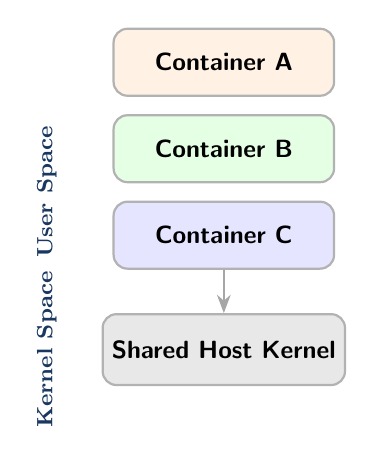
\begin{tikzpicture}[
    font=\small\sffamily,
    container/.style={draw=gray!60, rounded corners=5pt, thick, minimum width=2.8cm, minimum height=0.85cm, align=center},
    kernel/.style={draw=gray!60, fill=gray!18, rounded corners=5pt, thick, minimum width=3cm, minimum height=0.9cm, align=center},
]
\node[container, fill=orange!10] (c1) {\textbf{Container A}};
\node[container, fill=green!10, below=0.22cm of c1] (c2) {\textbf{Container B}};
\node[container, fill=blue!10, below=0.22cm of c2] (c3) {\textbf{Container C}};
\node[kernel, below=0.55cm of c3] (k) {\textbf{Shared Host Kernel}};

\draw[-{Stealth}, thick, gray!70] (c3.south) -- (k.north);

\node[rotate=90, font=\footnotesize\bfseries, text=SJCETblue, anchor=south] at ($(c2)!0.5!(c3) + (-2cm,0)$) {User Space};
\node[rotate=90, font=\footnotesize\bfseries, text=SJCETblue, anchor=south] at ($(k) + (-2cm,0)$) {Kernel Space};
\end{tikzpicture}
\end{column}
\end{columns}
\end{frame}

\begin{frame}{The Basic Idea Behind DeSFAM}
DeSFAM learns which syscalls a workload genuinely needs, watches live behaviour for anomalies, and enforces decisions directly inside the kernel --- without restarting the container.

\vspace{0.35cm}
\begin{columns}[T,onlytextwidth]
\begin{column}{0.32\textwidth}
\centering

\begin{tikzpicture}[scale=0.9]
\draw[SJCETblue, fill=SJCETblue!15, thick, rounded corners=2pt] (0,0) -- (1,0) -- (1,1.2) -- (0.5,1.6) -- (0,1.2) -- cycle;
\draw[SJCETblue, thick] (0.2,0.9) -- (0.8,0.9);
\draw[SJCETblue, thick] (0.2,0.6) -- (0.8,0.6);
\draw[SJCETblue, thick] (0.2,0.3) -- (0.6,0.3);
\end{tikzpicture}\\[0.15cm]
\textbf{1. Hybrid Syscall Listing}\\[0.1cm]
\footnotesize
Static call-graph analysis + live eBPF tracing builds a minimal per-container allow-list.
\end{column}

\begin{column}{0.32\textwidth}
\centering

\begin{tikzpicture}[scale=0.9]
\draw[SJCETblue, thick] (0.5,1.5) circle (0.35);
\draw[SJCETblue, thick] (0.5,1.15) -- (0.5,0.7);
\draw[SJCETblue, thick] (0.5,0.7) -- (0.2,0.3);
\draw[SJCETblue, thick] (0.5,0.7) -- (0.8,0.3);
\draw[SJCETblue, thick] (0.35,0.95) -- (0.65,0.95);
\end{tikzpicture}\\[0.15cm]
\textbf{2. AI-Driven Watching}\\[0.1cm]
\footnotesize
SyscallAD pairs a Variational Autoencoder with an Isolation Forest to spot broken patterns.
\end{column}

\begin{column}{0.32\textwidth}
\centering

\begin{tikzpicture}[scale=0.9]
\draw[SJCETblue, fill=SJCETblue!15, thick, rounded corners=3pt] (0,0) -- (1,0) -- (1,1.1) -- (0.5,1.5) -- (0,1.1) -- cycle;
\draw[SJCETblue, fill=white, thick] (0.5,0.75) circle (0.18);
\draw[SJCETblue, thick] (0.32,0.75) -- (0.32,0.35) -- (0.68,0.35) -- (0.68,0.75);
\fill[SJCETblue] (0.5,0.7) circle (0.06);
\draw[SJCETblue, thick] (0.5,0.7) -- (0.5,0.5);
\end{tikzpicture}\\[0.15cm]
\textbf{3. In-Kernel Enforcement}\\[0.1cm]
\footnotesize
eBPF programs at LSM hooks block, throttle, or log risky calls the instant they happen.
\end{column}
\end{columns}

\vspace{0.4cm}
\centering
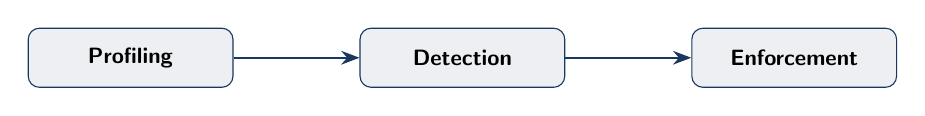
\begin{tikzpicture}[font=\footnotesize\sffamily, node distance=1.6cm,
    box/.style={draw=SJCETblue, rounded corners, fill=SJCETblue!8, minimum width=2.6cm, minimum height=0.75cm, align=center}]
\node[box] (a) {\textbf{Profiling}};
\node[box, right=of a] (b) {\textbf{Detection}};
\node[box, right=of b] (c) {\textbf{Enforcement}};
\draw[-{Stealth}, thick, SJCETblue] (a) -- (b);
\draw[-{Stealth}, thick, SJCETblue] (b) -- (c);
\end{tikzpicture}
\end{frame}

%==============================================================================
\section{Literature Survey}
%==============================================================================

\begin{frame}{Papers Covered}
\centering
\renewcommand{\arraystretch}{1.4}
\begin{tabular}{@{}clcc@{}}
\toprule
\textbf{\#} & \textbf{Paper} & \textbf{Year} & \textbf{Publisher} \\
\midrule
1 & DeSFAM & 2025 & IEEE Access \\
2 & Confine & 2023 & Computers \& Security \\
3 & Prof-gen & 2021 & IEEE CLOUD \\
4 & Optimus & 2024 & J. Cloud Computing \\
5 & KubeRosy & 2024 & IEEE Access \\
6 & PACED & 2022 & IEEE IC2E \\
7 & Condo & 2024 & IEEE TIFS \\
\bottomrule
\end{tabular}
\end{frame}

%------------------------------------------------------------------------------
% PAPER 1
%------------------------------------------------------------------------------
\begin{frame}{Paper 1}
\vspace{0.4cm}
\begin{center}
{\Large\bfseries DeSFAM: Adaptive eBPF \& AI-Driven Container Security}\\[0.15cm]
{\small\color{DarkGray}\textit{S. Zehra, H. J. Syed, F. Samad, U. Faseeha} | IEEE Access | 2025}
\end{center}

\vspace{0.2cm}
{\small Combines a hybrid syscall allow-list, an AI anomaly detector (SyscallAD), and eBPF/LSM enforcement to secure containers in real time.}

\vspace{0.2cm}
\begin{columns}[T,onlytextwidth]
\begin{column}{0.48\textwidth}
\begin{tcolorbox}[colback=green!5,colframe=green!50!black,title={\textcolor{green!50!black}{\faCheckCircle}~Where It Wins},fonttitle=\bfseries\small,boxrule=0.5pt,arc=2mm,left=2mm,right=2mm,top=1mm,bottom=1mm]
\footnotesize
\begin{itemize}
  \item eBPF + LSM hooks enforce decisions directly inside the kernel.
  \item VAE + Isolation Forest ensemble catches sequence-level anomalies.
\end{itemize}
\end{tcolorbox}
\end{column}

\begin{column}{0.48\textwidth}
\begin{tcolorbox}[colback=red!5,colframe=red!50!black,title={\textcolor{red}{\faTimesCircle}~Where It Struggles},fonttitle=\bfseries\small,boxrule=0.5pt,arc=2mm,left=2mm,right=2mm,top=1mm,bottom=1mm]
\footnotesize
\begin{itemize}
  \item Requires a well-labelled dataset (DongTing) for training.
  \item Three coordinated phases add deployment complexity.
\end{itemize}
\end{tcolorbox}
\end{column}
\end{columns}
\end{frame}

%------------------------------------------------------------------------------
% PAPER 2
%------------------------------------------------------------------------------
\begin{frame}{Paper 2}
\vspace{0.4cm}
\begin{center}
{\Large\bfseries Confine: Fine-Grained System Call Filtering}\\[0.15cm]
{\small\color{DarkGray}\textit{M. Rostamipoor, S. Ghavamnia, M. Polychronakis} | Computers \& Security | 2023}
\end{center}

\vspace{0.2cm}
{\small Performs static call-graph analysis on container binaries and compiles the result into a restrictive seccomp-BPF profile.}

\vspace{0.2cm}
\begin{columns}[T,onlytextwidth]
\begin{column}{0.48\textwidth}
\begin{tcolorbox}[colback=green!5,colframe=green!50!black,title={\textcolor{green!50!black}{\faCheckCircle}~Where It Wins},fonttitle=\bfseries\small,boxrule=0.5pt,arc=2mm,left=2mm,right=2mm,top=1mm,bottom=1mm]
\footnotesize
\begin{itemize}
  \item Purely static; adds zero runtime tracing overhead.
  \item Profiles plug directly into Docker's seccomp-BPF filtering.
\end{itemize}
\end{tcolorbox}
\end{column}

\begin{column}{0.48\textwidth}
\begin{tcolorbox}[colback=red!5,colframe=red!50!black,title={\textcolor{red}{\faTimesCircle}~Where It Struggles},fonttitle=\bfseries\small,boxrule=0.5pt,arc=2mm,left=2mm,right=2mm,top=1mm,bottom=1mm]
\footnotesize
\begin{itemize}
  \item seccomp checks one syscall at a time, missing sequences.
  \item Generated profile cannot adapt if app behaviour changes.
\end{itemize}
\end{tcolorbox}
\end{column}
\end{columns}
\end{frame}

%------------------------------------------------------------------------------
% PAPER 3
%------------------------------------------------------------------------------
\begin{frame}{Paper 3}
\vspace{0.4cm}
\begin{center}
{\Large\bfseries Prof-gen: Practical Syscall Whitelist Generation}\\[0.15cm]
{\small\color{DarkGray}\textit{S. Kim, B. J. Kim, D. H. Lee} | IEEE CLOUD | 2021}
\end{center}

\vspace{0.2cm}
{\small Traces a container through boot-time execution and cross-checks it against a static call graph to build a minimal whitelist.}

\vspace{0.2cm}
\begin{columns}[T,onlytextwidth]
\begin{column}{0.48\textwidth}
\begin{tcolorbox}[colback=green!5,colframe=green!50!black,title={\textcolor{green!50!black}{\faCheckCircle}~Where It Wins},fonttitle=\bfseries\small,boxrule=0.5pt,arc=2mm,left=2mm,right=2mm,top=1mm,bottom=1mm]
\footnotesize
\begin{itemize}
  \item Needs no source code --- works on binary-only images.
  \item Cross-checking keeps whitelists compact and accurate.
\end{itemize}
\end{tcolorbox}
\end{column}

\begin{column}{0.48\textwidth}
\begin{tcolorbox}[colback=red!5,colframe=red!50!black,title={\textcolor{red}{\faTimesCircle}~Where It Struggles},fonttitle=\bfseries\small,boxrule=0.5pt,arc=2mm,left=2mm,right=2mm,top=1mm,bottom=1mm]
\footnotesize
\begin{itemize}
  \item Whitelist is frozen after generation; no runtime updates.
  \item Boot-time tracing misses rarely triggered code paths.
\end{itemize}
\end{tcolorbox}
\end{column}
\end{columns}
\end{frame}

%------------------------------------------------------------------------------
% PAPER 4
%------------------------------------------------------------------------------
\begin{frame}{Paper 4}
\vspace{0.4cm}
\begin{center}
{\Large\bfseries Optimus: Association-Based Dynamic Filtering}\\[0.15cm]
{\small\color{DarkGray}\textit{S. Yang, B. B. Kang, J. Nam} | J. Cloud Computing | 2024}
\end{center}

\vspace{0.2cm}
{\small Uses eBPF to trace live syscalls, then applies association-rule mining to learn which calls typically occur together.}

\vspace{0.2cm}
\begin{columns}[T,onlytextwidth]
\begin{column}{0.48\textwidth}
\begin{tcolorbox}[colback=green!5,colframe=green!50!black,title={\textcolor{green!50!black}{\faCheckCircle}~Where It Wins},fonttitle=\bfseries\small,boxrule=0.5pt,arc=2mm,left=2mm,right=2mm,top=1mm,bottom=1mm]
\footnotesize
\begin{itemize}
  \item Profile adapts after deployment instead of staying fixed.
  \item Learns associations automatically, without hand-written rules.
\end{itemize}
\end{tcolorbox}
\end{column}

\begin{column}{0.48\textwidth}
\begin{tcolorbox}[colback=red!5,colframe=red!50!black,title={\textcolor{red}{\faTimesCircle}~Where It Struggles},fonttitle=\bfseries\small,boxrule=0.5pt,arc=2mm,left=2mm,right=2mm,top=1mm,bottom=1mm]
\footnotesize
\begin{itemize}
  \item Unmatched syscalls require manual operator approval.
  \item Updates halt entirely if association mining fails.
\end{itemize}
\end{tcolorbox}
\end{column}
\end{columns}
\end{frame}

%------------------------------------------------------------------------------
% PAPER 5
%------------------------------------------------------------------------------
\begin{frame}{Paper 5}
\vspace{0.4cm}
\begin{center}
{\Large\bfseries KubeRosy: Dynamic Filtering for Containers}\\[0.15cm]
{\small\color{DarkGray}\textit{J. Her, C. H. Jo, T. Park, S. Lee} | IEEE Access | 2024}
\end{center}

\vspace{0.2cm}
{\small Runs eBPF probes for live syscall monitoring and pushes policy changes through Kubernetes Custom Resource Definitions.}

\vspace{0.2cm}
\begin{columns}[T,onlytextwidth]
\begin{column}{0.48\textwidth}
\begin{tcolorbox}[colback=green!5,colframe=green!50!black,title={\textcolor{green!50!black}{\faCheckCircle}~Where It Wins},fonttitle=\bfseries\small,boxrule=0.5pt,arc=2mm,left=2mm,right=2mm,top=1mm,bottom=1mm]
\footnotesize
\begin{itemize}
  \item Policy updates apply cluster-wide with no image rebuild.
  \item Fits naturally into existing Kubernetes operator workflows.
\end{itemize}
\end{tcolorbox}
\end{column}

\begin{column}{0.48\textwidth}
\begin{tcolorbox}[colback=red!5,colframe=red!50!black,title={\textcolor{red}{\faTimesCircle}~Where It Struggles},fonttitle=\bfseries\small,boxrule=0.5pt,arc=2mm,left=2mm,right=2mm,top=1mm,bottom=1mm]
\footnotesize
\begin{itemize}
  \item Built entirely around Kubernetes; unusable on standalone Docker.
  \item Adds dependency on CRDs and cluster-level components.
\end{itemize}
\end{tcolorbox}
\end{column}
\end{columns}
\end{frame}

%------------------------------------------------------------------------------
% PAPER 6
%------------------------------------------------------------------------------
\begin{frame}{Paper 6}
\vspace{0.4cm}
\begin{center}
{\Large\bfseries PACED: Provenance-Based Escape Detection}\\[0.15cm]
{\small\color{DarkGray}\textit{M. Abbas, S. Khan, A. Monum, et al.} | IEEE IC2E | 2022}
\end{center}

\vspace{0.2cm}
{\small Builds a provenance graph linking syscalls across containers and matches graph patterns to known escape techniques.}

\vspace{0.2cm}
\begin{columns}[T,onlytextwidth]
\begin{column}{0.48\textwidth}
\begin{tcolorbox}[colback=green!5,colframe=green!50!black,title={\textcolor{green!50!black}{\faCheckCircle}~Where It Wins},fonttitle=\bfseries\small,boxrule=0.5pt,arc=2mm,left=2mm,right=2mm,top=1mm,bottom=1mm]
\footnotesize
\begin{itemize}
  \item Captures multi-step, cross-container attack chains.
  \item Well suited to catching cross-namespace escape attempts.
\end{itemize}
\end{tcolorbox}
\end{column}

\begin{column}{0.48\textwidth}
\begin{tcolorbox}[colback=red!5,colframe=red!50!black,title={\textcolor{red}{\faTimesCircle}~Where It Struggles},fonttitle=\bfseries\small,boxrule=0.5pt,arc=2mm,left=2mm,right=2mm,top=1mm,bottom=1mm]
\footnotesize
\begin{itemize}
  \item Continuous graph construction is compute-intensive.
  \item Overhead grows with the number of containers tracked.
\end{itemize}
\end{tcolorbox}
\end{column}
\end{columns}
\end{frame}

%------------------------------------------------------------------------------
% PAPER 7
%------------------------------------------------------------------------------
\begin{frame}{Paper 7}
\vspace{0.4cm}
\begin{center}
{\Large\bfseries Condo: Kernel Permission Data Protection}\\[0.15cm]
{\small\color{DarkGray}\textit{S. Xu, Y. Wang, L. Lei, et al.} | IEEE TIFS | 2024}
\end{center}

\vspace{0.2cm}
{\small Protects kernel permission data using a hardware-backed Trusted Execution Environment (TEE), guarding against kernel-level tampering.}

\vspace{0.2cm}
\begin{columns}[T,onlytextwidth]
\begin{column}{0.48\textwidth}
\begin{tcolorbox}[colback=green!5,colframe=green!50!black,title={\textcolor{green!50!black}{\faCheckCircle}~Where It Wins},fonttitle=\bfseries\small,boxrule=0.5pt,arc=2mm,left=2mm,right=2mm,top=1mm,bottom=1mm]
\footnotesize
\begin{itemize}
  \item Hardware-rooted protection survives kernel compromise.
  \item Targets permission-data tampering that filters don't cover.
\end{itemize}
\end{tcolorbox}
\end{column}

\begin{column}{0.48\textwidth}
\begin{tcolorbox}[colback=red!5,colframe=red!50!black,title={\textcolor{red}{\faTimesCircle}~Where It Struggles},fonttitle=\bfseries\small,boxrule=0.5pt,arc=2mm,left=2mm,right=2mm,top=1mm,bottom=1mm]
\footnotesize
\begin{itemize}
  \item Requires TEE-capable hardware (Intel SGX / ARM TrustZone).
  \item Needs kernel modifications, raising the adoption bar.
\end{itemize}
\end{tcolorbox}
\end{column}
\end{columns}
\end{frame}

%------------------------------------------------------------------------------
% COMPARISON TABLE
%------------------------------------------------------------------------------
\begin{frame}{Technique Comparison}
\small
Compared by technique used, not by a single headline number.

\vspace{0.2cm}
\centering
\renewcommand{\arraystretch}{1.4}
\begin{tabular}{@{}lccccc@{}}
\toprule
 & \textbf{Static} & \textbf{Live eBPF} & \textbf{AI / ML} & \textbf{In-Kernel} & \textbf{Hardware} \\
 & \textbf{Analysis} & \textbf{Tracing} & \textbf{Detection} & \textbf{Enforcement} & \textbf{Isolation} \\
\midrule
\textbf{1. DeSFAM}   & \faCheck & \faCheck & \faCheck & \faCheck & --- \\
\textbf{2. Confine}    & \faCheck & ---      & ---      & ---      & --- \\
\textbf{3. Prof-gen}   & \faCheck & \faCheck & ---      & ---      & --- \\
\textbf{4. Optimus}    & ---      & \faCheck & ---      & ---      & --- \\
\textbf{5. KubeRosy}   & ---      & \faCheck & ---      & \faCheck & --- \\
\textbf{6. PACED}      & ---      & \faCheck & ---      & ---      & --- \\
\textbf{7. Condo}      & ---      & ---      & ---      & \faCheck & \faCheck \\
\bottomrule
\end{tabular}
\end{frame}

%==============================================================================
\section{Conclusion}
%==============================================================================

\begin{frame}{Conclusion: One Framework, Every Layer Covered}
\begin{columns}[T,onlytextwidth]
\begin{column}{0.58\textwidth}
\begin{block}{Key Insight}
Each prior paper contributes one piece --- static profiling, live eBPF adaptation, provenance analysis, or hardware isolation --- but \textbf{none combines them}.
\end{block}

\vspace{0.25cm}
\textbf{DeSFAM unifies:}
\begin{itemize}
  \item \textbf{Hybrid profiling} (static + dynamic analysis)
  \item \textbf{AI-driven detection} (VAE + Isolation Forest)
  \item \textbf{In-kernel enforcement} (eBPF + LSM hooks)
\end{itemize}

\vspace{0.2cm}
{\small into a single adaptive, real-time framework.}
\end{column}

\begin{column}{0.40\textwidth}
\centering
\vspace{0.3cm}
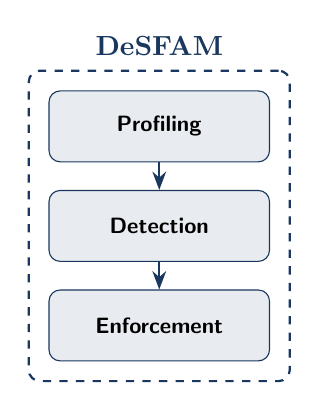
\begin{tikzpicture}[font=\footnotesize\sffamily,
    layer/.style={draw=SJCETblue, rounded corners, fill=SJCETblue!10, minimum width=2.8cm, minimum height=0.9cm, align=center}]
\node[layer] (p) {\textbf{Profiling}};
\node[layer, below=0.35cm of p] (d) {\textbf{Detection}};
\node[layer, below=0.35cm of d] (e) {\textbf{Enforcement}};
\draw[-{Stealth}, thick, SJCETblue] (p) -- (d);
\draw[-{Stealth}, thick, SJCETblue] (d) -- (e);

\node[fit=(p)(d)(e), draw=SJCETblue, thick, dashed, rounded corners=4pt, inner sep=0.25cm] (box) {};
\node[above=0.05cm of box, font=\bfseries, SJCETblue] {DeSFAM};
\end{tikzpicture}
\end{column}
\end{columns}
\end{frame}

%------------------------------------------------------------------------------
% THANK YOU (Separate Slide)
%------------------------------------------------------------------------------
{
\setbeamertemplate{footline}{}
\begin{frame}[plain]

\vfill
\begin{center}
{\Huge\bfseries\textcolor{SJCETblue}{Thank You}}\\[0.6cm]
{\large Questions \& Discussion}\\[0.3cm]
{\normalsize\textcolor{SJCETgold}{DeSFAM --- Literature Review}}
\end{center}
\vfill

\end{frame}
}

%==============================================================================
\end{document}